\documentclass[12pt, a4paper]{article}
\usepackage{../../../myconfig} % Gọi file cấu hình từ ngoài gốc vào

% ==========================================
% BẮT ĐẦU NỘI DUNG TÀI LIỆU
% ==========================================
\begin{document}


% Truyền 3 tham số: {Nhãn cam} {Chữ to chính giữa} {Chữ ở góc phải Header}
\titlebox{Chủ đề: Hàm số}{Đường tiện cận}{Hàm số: Đường tiện cận}



\begin{center}
\begin{tikzpicture}[>=latex, scale=1]
    % 1. Hệ trục tọa độ
    \draw[->] (-4.5,0) -- (3.5,0) node[below] {\small $x$};
    \draw[->] (0,-4.5) -- (0,3.5) node[right] {\small $y$};
    \node[below left] at (0,0) {\small $O$};
    
    % 2. Vẽ đồ thị hàm số
    \draw[thick, samples=100, domain=-4.5:-1.45] 
        plot (\x, {(-\x+0.5)/(\x + 1)});
    \draw[thick, samples=100, domain=-0.65:3.5] 
         plot (\x, {(-\x+0.5)/(\x + 1)});
    
    % 3. Đường tiệm cận
    \draw[thick] (-1,-4.5) -- (-1,3.5);
    \draw[thick] (-4.5,-1) -- (3.5,-1) ;
    % 4. Đánh dấu các điểm
    \node[below left] at (0,-1) {\small $-1$};
    \node[below left] at (-1,0) {\small $-1$};
\end{tikzpicture}
\quad \quad \quad
\begin{tikzpicture}[>=latex, scale=0.8]
    % 1. Hệ trục tọa độ
    \draw[->] (-3.5,0) -- (5.5,0) node[below] {\small $x$};
    \draw[->] (0,-4.5) -- (0,4.5) node[right] {\small $y$};
    \node[below left] at (0,0) {\small $O$};
    
    % 2. Vẽ đồ thị hàm số
    \draw[thick, samples=100, domain=-2.5:1.75] 
        plot (\x, {\x-2 + 1/(\x -2)});
    \draw[thick, samples=100, domain=2.25:5] 
        plot (\x, {\x-2 + 1/(\x -2)});
    \draw[thick, samples=100, domain=-2.5:5] 
        plot (\x, {\x-2});
    
    % 4. Đường tiệm cận đứng
    \draw[thick] (2,-4.5) -- (2,4.5) ;
    
    % 5. Đánh dấu các điểm
    \node[above left] at (1,0) {\small $1$};
     \node[above left] at (2,0) {\small $2$};
      \node[above left] at (0,-2) {\small $-2$};
    \draw [dashed] (1,0) -- (1,-2) -- (0,-2);
\end{tikzpicture}
\end{center}

\drawdashlines{10}
\newpage
\drawdashlines{25}
\newpage

\questionLinesManual{4}{1}{Cho hàm số \( y = \dfrac{ax + b}{cx + d} \) (\( c \neq 0 \), \( ad - bc \neq 0 \)) có đồ thị như hình vẽ bên. Tiệm cận ngang của đồ thị hàm số là:

\begin{center}
\begin{tikzpicture}[>=latex, scale=1]
    % 1. Hệ trục tọa độ
    \draw[->] (-3.5,0) -- (3.5,0) node[below] {\small $x$};
    \draw[->] (0,-3.5) -- (0,3.5) node[right] {\small $y$};
    \node[below left] at (0,0) {\small $O$};
    
    % 2. Vẽ đồ thị hàm số
    \draw[thick, samples=100, domain=-3.5:-1.13] 
        plot (\x, {0.5 + 0.5/(\x + 1)});
    \draw[thick, samples=100, domain=-0.83:3.5] 
        plot (\x, {0.5 + 0.5/(\x + 1)});
    
    % 3. Đường tiệm cận
    \draw[thick] (-1,-3.5) -- (-1,3.5) ;
    \draw[thick] (-3.5,0.5) -- (3.5,0.5) ;
    
    % 4. Đánh dấu các điểm
    \node[above left] at (0,0.5) {\small $\frac{1}{2}$};
    \node[below left] at (-1,0) {\small $-1$};
\end{tikzpicture}
\end{center}
}

\questionLinesManual{4}{2}{Hàm số \( y = \dfrac{ax + b}{cx + d} \) (\( c \neq 0 \), \( ad - bc \neq 0 \)) có đồ thị dưới đây. Đường tiệm cận đứng của đồ thị hàm số là:

\begin{center}
\begin{tikzpicture}[>=latex, scale=1]
    % 1. Hệ trục tọa độ
    \draw[->] (-3.5,0) -- (6.5,0) node[below] {\small $x$};
    \draw[->] (0,-3.5) -- (0,4.5) node[right] {\small $y$};
    \node[below left] at (0,0) {\small $O$};
    
    % 2. Vẽ đồ thị hàm số
    \draw[thick, samples=100, domain=-3.5:1.81] 
        plot (\x, {(-\x+1)/(\x -2) });
    \draw[thick, samples=100, domain=2.39:6.5] 
         plot (\x, {(-\x+1)/(\x -2) });
    
    % 3. Đường tiệm cận
    \draw[dashed] (2,-3.5) -- (2,4.5) ;
    \draw[dashed] (-3.5,-1) -- (6.5,-1) ;
    
    % 4. Đánh dấu các điểm
    \node[ below left] at (0,-1) {\small $-1$};
    \node[below right] at (1,0) {\small $1$};
    \node[below right] at (2,0) {\small $2$};
    \filldraw (2,0) circle (1.5pt);
    \filldraw (1,0) circle (1.5pt);
    \filldraw (0,-1) circle (1.5pt);
\end{tikzpicture}
\end{center}}

\questionLinesManual{10}{3}{Cho hàm số \( y = f(x) \) có đồ thị như hình vẽ:

\begin{center}
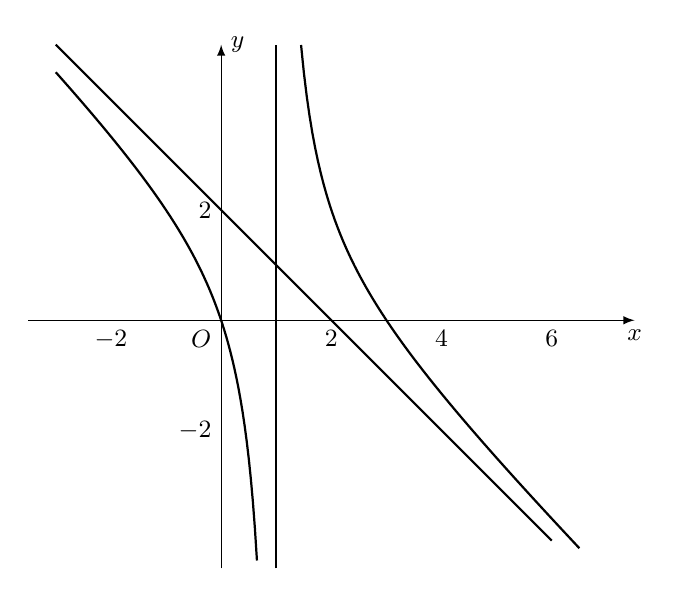
\begin{tikzpicture}[>=latex, scale=0.7]
    % 1. Hệ trục tọa độ
    \draw[->] (-3.5,0) -- (7.5,0) node[below] {\small $x$};
    \draw[->] (0,-4.5) -- (0,5) node[right] {\small $y$};
    \node[below left] at (0,0) {\small $O$};
    
    % 2. Vẽ đồ thị hàm số
    \draw[thick, samples=100, domain=-3:0.65] 
        plot (\x, {-\x+2 + 2/(\x -1)});
    \draw[thick, samples=100, domain=1.45:6.5] 
        plot (\x, {-\x+2 + 2/(\x -1)});
    \draw[thick, samples=100, domain=-3:6] 
        plot (\x, {-\x+2 });
    % 3. Đường tiệm cận
    \draw[thick] (1,-4.5) -- (1,5) ;
   
    
    % 4. Đánh dấu các điểm
    \node[left] at (0,-2) {\small $-2$};
     \node[left] at (0,2) {\small $2$};
    \node[below] at (-2,0) {\small $-2$};
    \node[below] at (2,0) {\small $2$};
    \node[below] at (4,0) {\small $4$};
    \node[below] at (6,0) {\small $6$};
\end{tikzpicture}
\end{center}

Đồ thị hàm số đã cho có bao nhiêu đường tiệm cận, phương trình cuaur các đường tiệm cận đó?}

\questionLinesManual{14}{4}{Cho hàm số \( y = f(x) \) có đồ thị hàm số như hình sau:

\begin{center}
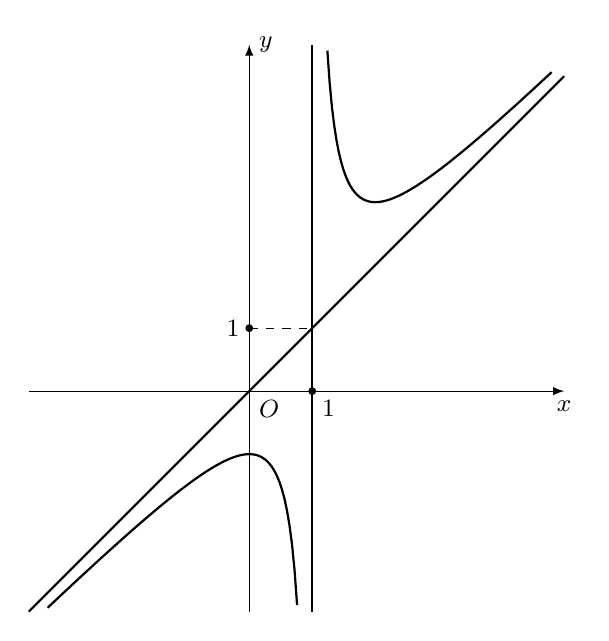
\begin{tikzpicture}[>=latex, scale=0.8]
    % 1. Hệ trục tọa độ
    \draw[->] (-3.5,0) -- (5,0) node[below] {\small $x$};
    \draw[->] (0,-3.5) -- (0,5.5) node[right] {\small $y$};
    \node[below right] at (0,0) {\small $O$};
    
    % 2. Vẽ đồ thị hàm số (có tiệm cận xiên y = x - 1)
    \draw[thick, samples=100, domain=-3.2:0.76] 
        plot (\x, {\x  + 1/(\x-1)});
    \draw[thick, samples=100, domain=1.24:4.8] 
        plot (\x, {\x  + 1/(\x-1)});
    \draw[thick, samples=100, domain=-3.5:5] 
        plot (\x, {\x  });
    % 4. Đường tiệm cận đứng
    \draw[thick] (1,-3.5) -- (1,5.5);
    \draw[dashed] (0,1)--(1,1);
    % 5. Đánh dấu các điểm
   
    \node[below right] at (1,0) {\small $1$};
    \node[left] at (0,1) {\small $1$};
    \filldraw (1,0) circle (1.5pt);
    \filldraw (0,1) circle (1.5pt);
\end{tikzpicture}
\end{center}

Đường tiệm cận xiên của đồ thị hàm số là}

\questionLinesManual{10}{5}{Cho hàm số \( y = \dfrac{ax + b}{cx + d} \) (\( c \neq 0; ad - bc \neq 0 \)) có đồ thị như hình vẽ bên dưới.

\begin{center}
\begin{tikzpicture}[>=latex, scale=1]
    % 1. Hệ trục tọa độ
    \draw[->] (-3.5,0) -- (5.5,0) node[below] {\small $x$};
    \draw[->] (0,-3.5) -- (0,2.5) node[right] {\small $y$};
    \node[below left] at (0,0) {\small $O$};
    
    % 2. Vẽ đồ thị hàm số
    \draw[thick, samples=100, domain=-3.5:0.6] 
        plot (\x, {(-\x+2)/(\x - 1)});
    \draw[thick, samples=100, domain=1.3:5.5] 
        plot (\x, {(-\x+2)/(\x - 1)});
    
    % 3. Đường tiệm cận
    \draw[thick] (1,-3.5) -- (1,2.5);
    \draw[thick] (-3.5,-1) -- (5.5,-1);
    
    % 4. Đánh dấu các điểm
    \node[ below left] at (0,-1) {\small $-1$};
    \node[below left] at (1,0) {\small $1$};
     \node[below] at (2,0) {\small $2$};
      \node[below] at (0,-2) {\small $-2$};
    \filldraw (1,0) circle (1.5pt);
    \filldraw (2,0) circle (1.5pt);
    \filldraw (0,-1) circle (1.5pt);
    \filldraw (0,-2) circle (1.5pt);
\end{tikzpicture}
\end{center}

Đồ thị hàm số có đường tiệm cận ngang là:}{
    \begin{tasks}(4)
        \task \( y = 0 \)
        \task \( y = -1 \)
        \task \( x = -1 \)
        \task \( y = 1 \)
    \end{tasks}
}

% --- CÂU 52 ---
\questionLinesManual{10}{6}{Cho hàm số \( y = \dfrac{ax^2 + bx + c}{mx + n} \) có đồ thị như hình bên.

\begin{center}
\begin{tikzpicture}[>=latex, scale=1]
    % 1. Hệ trục tọa độ
    \draw[->] (-4.5,0) -- (4.5,0) node[below] {\small $x$};
    \draw[->] (0,-4.5) -- (0,4.5) node[right] {\small $y$};
    \node[below left] at (0,0) {\small $O$};
    
    % 2. Vẽ đồ thị hàm số
    \draw[thick, samples=100, domain=-4:-1.25] 
        plot (\x, {-\x - 1 + -1/(\x + 1)});
     \draw[thick, samples=100, domain=-0.75:3] 
        plot (\x, {-\x - 1 + -1/(\x + 1)});
     \draw[thick, samples=100, domain=-4:3] 
        plot (\x, {-\x - 1});
    \draw[thick] (-1,-4.5) -- (-1,4.5) ;
    
    % 5. Đánh dấu các điểm
    \node[below left] at (-1,0) {\small $-1$};
    \node[below] at (1,0) {\small $1$};
    \node[below left] at (0,-1) {\small $-1$};
    \filldraw (-1,0) circle (1.5pt);
    \filldraw (1,0) circle (1.5pt);
    \filldraw (0,-1) circle (1.5pt);
\end{tikzpicture}
\end{center}

Tiệm cận xiên của đồ thị hàm số đã cho là}{
    \begin{tasks}(4)
        \task \( y = -x + 1 \)
        \task \( y = x - 1 \)
        \task \( y = -x - 1 \)
        \task \( y = x + 1 \)
    \end{tasks}
}

\newpage
\drawdashlines{25}
\newpage

\questionLinesManual{5}{7}{Tiệm cận của đồ thị hàm số \( y = \dfrac{2x - 3}{x + 1} \) là đường thẳng có phương trình}
 
\questionLinesManual{5}{8}{Tiệm cận của đồ thị hàm số \( y = \dfrac{x - 1}{x - 3} \) là}

\questionLinesManual{7}{9}{Đường tiệm cận ngang của đồ thị hàm số \( y = 1 + \dfrac{2x + 1}{x + 2} \) có phương trình là:}

\questionLinesManual{8}{10}{Cho đồ thị hàm số \( y = \dfrac{2x^2 + x - 5}{x + 3} \) có đường tiệm cận xiên là đường thẳng \( \Delta : y = ax + b \) với \( a, b \in \mathbb{R}, a \neq 0 \). Giá trị của tổng \( a + b \) bằng}

\questionLinesManual{8}{11}{Đường tiệm cận xiên của đồ thị hàm số \( y = \dfrac{x^2 + 2x - 3}{x - 2} \) là}

\questionLinesManual{9}{12}{Đường tiệm cận xiên của đồ thị hàm số \( y = 2x - 1 + \dfrac{1}{x} \) có phương trình là:}

\questionLinesManual{8}{13}{Đồ thị hàm số \( y = 2x + 1 - \dfrac{3}{x + 1} \) có đường tiệm cận xiên là:}

\questionLinesManual{8}{14}{Cho hàm số \( y = 2x - 1 - \dfrac{3}{x + 2} \). Đường tiệm cận xiên của đồ thị hàm số đã cho là:}

\questionLinesManual{12}{15}{Cho hàm số \( y = \dfrac{ax + b}{cx + d} \), (\(ac \neq 0, ad - bc \neq 0\)) có bảng biến thiên như dưới đây.

\begin{center}

\begin{tikzpicture}
    \tkzTabInit[lgt=1.5, espcl=3.5]
    {$x$ /1, $y'$ /1, $y$ /2.5}
    {$-\infty$, $-2$, $+\infty$}
    \tkzTabLine{, -, d, -, }
    \tkzTabVar{+/ $1$ / , -D+/ $-\infty$ / $+\infty$ , -/ $1$ /}
\end{tikzpicture}
\end{center}

Đường tiệm cận đứng của đồ thị hàm số đã cho có phương trình là}

\questionLinesManual{8}{16}{Cho hàm số \( y = f(x) \) có bảng biến thiên như hình vẽ dưới đây.

\begin{center}

\begin{tikzpicture}
    \tkzTabInit[lgt=1.5, espcl=3.5]
    {$x$ /1, $y'$ /1, $y$ /2.5}
    {$-\infty$, $1$, $2$, $+\infty$}
    \tkzTabLine{, -, d, -, 0, +, }
    \tkzTabVar{+/ $-1$ / , -D+/ $-\infty$ / $+\infty$ , -/ $1$ / , +/ $2$ /}
\end{tikzpicture}
\end{center}

Đồ thị hàm số \( y = f(x) \) có bao nhiêu đường tiệm cận?}

\questionLinesManual{5}{17}{Cho hàm số \( f(x) \) xác định trên \( (-\infty; 0) \setminus \{-2\} \) và có bảng biến thiên bên dưới. Đồ thị hàm số đã cho có tổng số đường tiệm cận ngang và tiệm cận đứng là

\begin{center}
\begin{tikzpicture}
    \tkzTabInit[lgt=1.5, espcl=3.5]
    {$x$ /1, $f'(x)$ /1, $f(x)$ /2.5}
    {$-\infty$, $-2$, $0$, $+\infty$}
    \tkzTabLine{, +, d, -, d,+}
    \tkzTabVar{-/ $-\infty$ / , +D+/ $+\infty$ / $1$, -D/ $0$ /}
   \fill[pattern=north east lines](9,-4.5) rectangle (13,-1);
\end{tikzpicture}
\end{center}}

\questionLinesManual{8}{18}{Cho hàm số \( y = f(x) \) có bảng biến thiên như sau:

\begin{center}

\begin{tikzpicture}
    \tkzTabInit[lgt=1.5, espcl=3.5]
    {$x$ /1, $y'$ /1, $y$ /2.5}
    {$-\infty$, $-3$, $3$, $+\infty$}
    \tkzTabLine{, +, d, +, d, +, }
    \tkzTabVar{-/ $0$ / , +D-/ $+\infty$ / $-\infty$, +D-/ $+\infty$ / $-\infty$, +/ $0$ /}
\end{tikzpicture}
\end{center}

Số đường tiệm cận đứng của đồ thị hàm số là}

\questionLinesManual{5}{19}{Cho hàm số \( y = f(x) \) có bảng biến thiên như sau

\begin{center}

\begin{tikzpicture}
    \tkzTabInit[lgt=1.5, espcl=2.5]
    {$x$ /1, $y'$ /1, $y$ /2.5}
    {$-\infty$, $-2$, $0$, $+\infty$}
    \tkzTabLine{, -, d, +, d, -, }
    \tkzTabVar{+/ $+\infty$ / , -D-/ $1$ / $-\infty$/ ,+D+/ $+\infty$ / $1$ , -/ $0$ /}
\end{tikzpicture}
\end{center}

Tổng số đường tiệm cận đứng và tiệm cận ngang của đồ thị hàm số đã cho bằng}


\questionLinesManual{15}{20}{Cho hàm số có bảng biến thiên như hình sau

\begin{center}

\begin{tikzpicture}
    \tkzTabInit[lgt=1.5, espcl=2.5]
    {$x$ /1, $y'$ /1, $y$ /2.5}
    {$-\infty$, $-1$, $0$, $1$, $+\infty$}
    \tkzTabLine{, +, d, +, d, -, d, +, }
    \tkzTabVar{-/ $-4$ / , +D-/ $+\infty$ /  $-\infty$,+ / $2$ ,  -D-/ $-\infty$ /$-\infty$ , +/ $-1$ /}
\end{tikzpicture}
\end{center}

Tổng số đường tiệm cận ngang và tiệm cận đứng của đồ thị hàm số \( y = f(x) \) là}

\newpage
\drawdashlines{25}
\end{document}